\chapter{Related work}\label{chapter:related_work}
In this chapter we describe the existing solutions for user study data collection. According to the problem statement in Section \ref{section:software} we list the usability data logging software which provides media recordings capturing, feedback forms and additional functionality to capture the data during the experiment. These software solutions might be used for the experiment data collection and analysis, although they have certain disadvantages. We also review alternative methods in Section \ref{section:alternative}, which means combining several solutions to fulfill the needed functionality. In both sections we explain how the experiment design and configuration, experiment flow and data analysis would look on an example. In Section \ref{section:distinction} we explain why our solution is better for the problem scope.\\   

\section{Usability data logging software}\label{section:software}
The market has a lot of commercial software solutions designed for usability data logging: Techsmith, OvoStudios, Bit Debris, Noldus, Usability Systems/Alucid. Most of them offer support recording, bookmarking, feedback forms and are designed for a wide market research of general software usability testing. We'll review to what extend these solutions can be adapted to the MaCon evaluation user study and how they cover the problem on the example of Techsmith/Morae.\\

\textbf{Morae} by Techsmith \cite{morae} is a Windows only solution for for analyzing human-computer interaction. It contains the functionality of capturing the recordings, marking Tasks and provides surveys. Some of the study configurations would be especially important for the study over the MaCon workbench. The researcher can disable the manual start/stop of the recordings so no important information would be lost. The main means of experiment work-flow decomposition are Tasks. The Tasks can be configurable and contain instructions. In the scope of the research the Tasks would represent the engineering process activities, for example requirements specification, test specification, etc. You can see the Task editing window on Figure \ref{fig:movae_tasks}. The researcher can also configure Markers to bookmark certain events like on the Figure \ref{fig:movae_markers}.\\

   \begin{figure}[htb]
 \centering
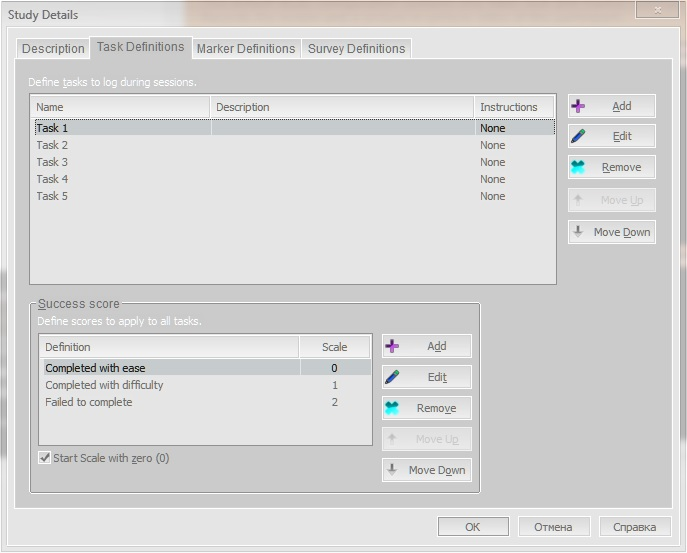
\includegraphics[width=\textwidth]{figures/movae_tasks.jpg}
\caption{Movae Tasks editing window}
\label{fig:movae_tasks}
 \end{figure}
 
    \begin{figure}[htb]
 \centering
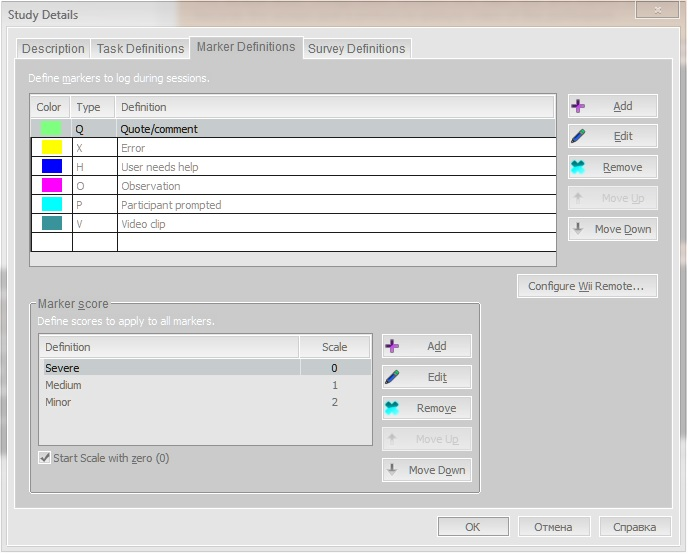
\includegraphics[width=\textwidth]{figures/movae_markers.jpg}
\caption{Movae Markers editing window}
\label{fig:movae_markers}
 \end{figure}

The software provides a sufficient flexibility to configure good surveys that would fit the MaCon evaluation study. The survey can be triggered by one of the following events: end of a Task, beginning or end of the recording. You can see the survey configuration window on Figure \ref{fig:movae_survey_1}.\\
 
    \begin{figure}[htb]
 \centering
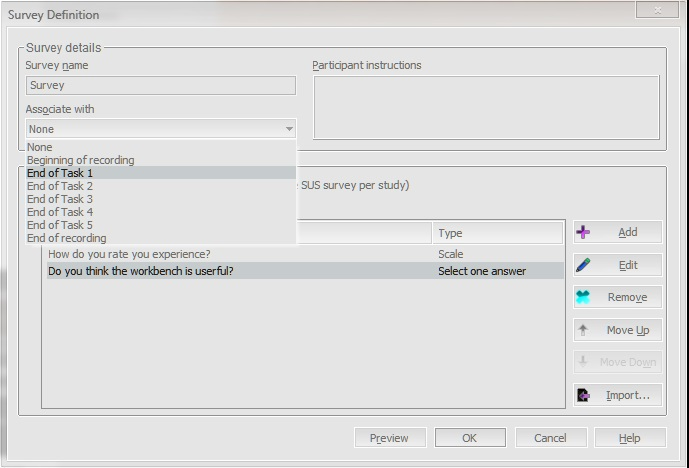
\includegraphics[width=\textwidth]{figures/movae_surveys_1.jpg}
\caption{Movae Survey editing window}
\label{fig:movae_survey_1}
 \end{figure}
 
 The researcher can configure questions of the following types: scale, text, single answer and multiple answer. The question configuration window is on the Figure \ref{fig:movae_survey_2}.\\
 
     \begin{figure}[htb]
 \centering
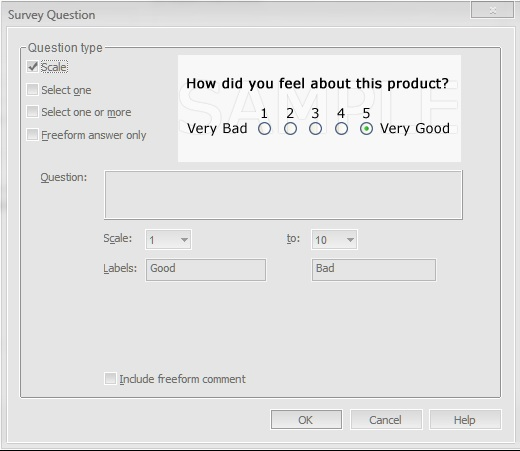
\includegraphics{figures/movae_surveys_2.jpg}
\caption{Movae Question editing window}
\label{fig:movae_survey_2}
 \end{figure}
 
 The researcher wouldn't have to configure every workstation, but can load the pre-saved configuration. During the experiment the participants would work with two pieces of software: MaCon workbench and Movae recorder, where they would answer to the Surveys and save Tasks and Markers accordingly to the experiment design.\\
 
 After the experiment the data would be analyzed in the Movae Manager (Figure \ref{fig:movae_manager}). The manager provides a video player for the recordings, functionality to search, filter information by Tasks and Markers as well as add new Markers and observations.The Manager provides data visualization of Tasks time and success rate and ability to export surveys data. \\
 
      \begin{figure}[htb]
 \centering
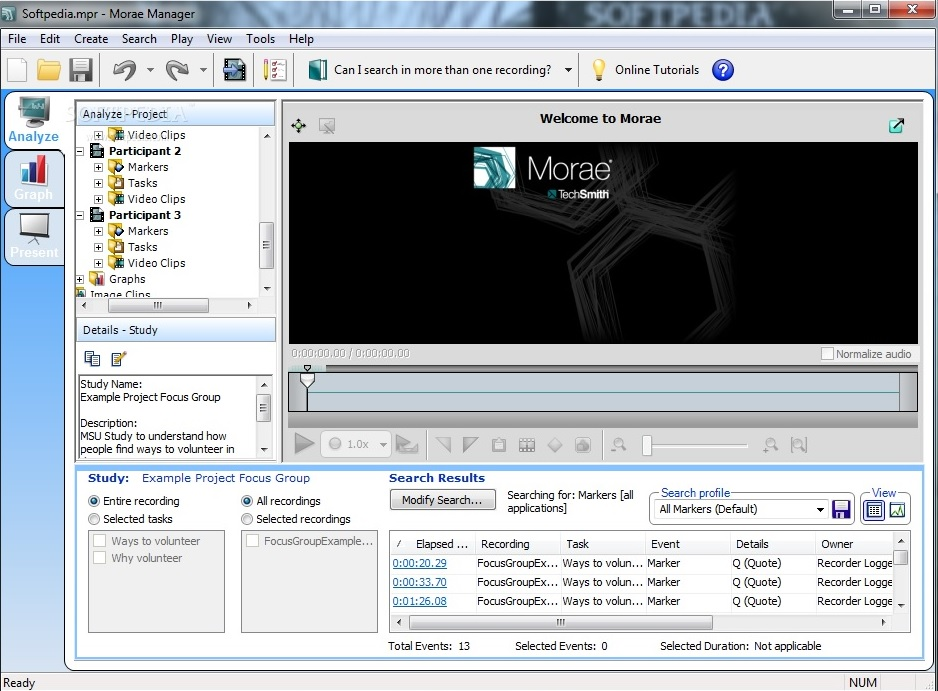
\includegraphics[width=\textwidth]{figures/morae_manager.jpg}
\caption{Morae Manager}
\label{fig:movae_manager}
 \end{figure}
 
 This approach would be possible for the evaluation study on MaCon approach, but it would have some disadvantages. Movae provides a lot of complicated functionality that is not needed for the study, but doesn't cover the following. Tasks are supposed to be sequential or independent and the software doesn't support folding or correlation of Tasks, thus usage of Tasks as engineering activities would be tricky if the engineering process is complicated. Surveys can be fired only at the start of Tasks, start or end of the recording, which doesn't cover the need of firing the survey in other situations like beginning of the task, saving some Marker (like Error), certain state of the system. Survey results are not displayed nor processed, so the researcher would have to use some other tools to study the questionnaires, thus the correlation between survey results and Tasks and Markers becomes a complicated issue. Most of all, the solution is not designed for retrospective analysis of parallel sessions. All session are considered as independent and the analysis of the project would require additional effort in synchronization of the sessions and recordings. This issue is especially important for the application domain in the case of concurrent engineering, which implies parallel work of several engineers on the same system design.\\ 

The commercial software solutions have multiple disadvantages for the common use:

\begin{itemize}
\item Expensive, ranging from a few hundred dollars to several thousand dollars.
\item Complex to learn and master depending on the product's feature list.
\item Limited to the PC platform.
\item Often focused primarily on the recording, storage, and retrieval of selected video data, with less attention paid to recording and analyzing observed data.
\item Lack of customization available.
\item Require significant hard drive space for installation.
\end{itemize}

Most of all unlike the solution presented in this thesis the commercial usability data loggers are not designed for evaluation of the engineering approaches therefore don't adjust to the manufacturing project development process, specific events like model simulation, process stages and milestones, collaborative work etc. As the standalone software solutions are not integrated to the workbench, the interaction with inner events of the workbench and inner workbench data is not possible.\\

The other mentioned software solutions provide quite similar functionality to the one provided by Morae, therefore would be used in the same way and provide same disadvantages.

\section{Alternative approaches}\label{section:alternative}

Also the components of the experiment data collection can be partially replaced by the combination of several software solution, like standalone recording software and paper surveys or Google forms, Typeform, etc. There are user studies that use such original means to collect user feedback as Sharepoint environment \cite{chp} or tape the oral interview and transkript the answers afterwards \cite{Kuhn2012}. We'll review  how the experiment could be conducted with the usage of Ovo Solo recording software.\\

OvoStudios provide a software solution called \textbf{Ovo Solo} for capturing and logging user interaction with a software. It captures screen, audio and video recording and is a standalone program with own interface. The solution provides three ways of submitting information for the study participants: Observation, Highlight and QuickLog. The main window of the software is on the Figure \ref{fig:ovosolo_main}. The information is submitted in a form shown on the Figure \ref{fig:ovosolo_note} and is called through Take Note button of the main menu. As you can see the user can either type a custom Observation, either select an predefined observation from the list of available QuickLog observations, either set start and end time for a recording clip Highlighting. \\ 

 \begin{figure}[htb]
 \centering
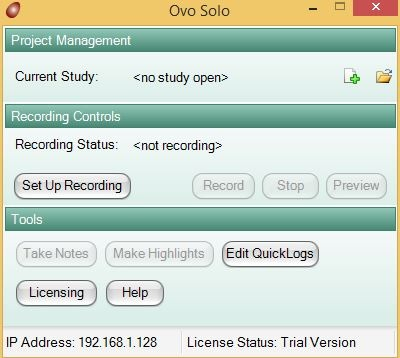
\includegraphics{figures/ovosolo_main.jpg}
\caption{Ovo Solo main window}
\label{fig:ovosolo_main}
 \end{figure}
 
  \begin{figure}[htb]
 \centering
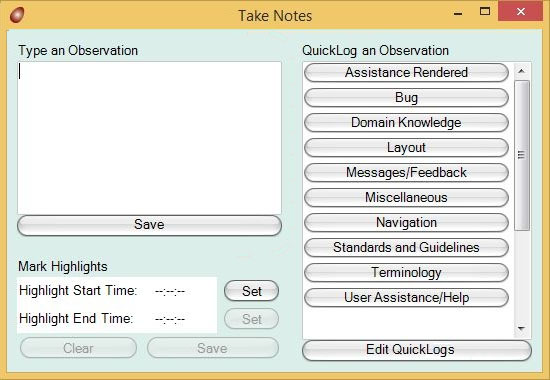
\includegraphics[width=\textwidth]{figures/ovosolo_note.jpg}
\caption{Ovo Solo note submission window}
\label{fig:ovosolo_note}
 \end{figure}
 
The MaCon evaluation study could use the tool in the following way. The researcher would install the software on every workstation and configure it by setting up the recording, which means selecting the input devices and enabling microphone, screen capturing and video recording and edit the QuickLog options to represent the available predefined observations.You can see the editing of the predefined observation options on Figure \ref{fig:ovosolo_edit}. During the experiment the user would have to use either the Highlighting, either the predefined QuickLog options to mark the development milestones and phases, which are important for the retrospective analysis for the evaluation of the approach. The participant would use the custom observations to leave the feedback. As the tool doesn't have the functionality for questionnaires, the surveys have to be done in some other way: online forms, like Google Forms, Typeform, etc, paper surveys, oral interview.\\

   \begin{figure}[htb]
 \centering
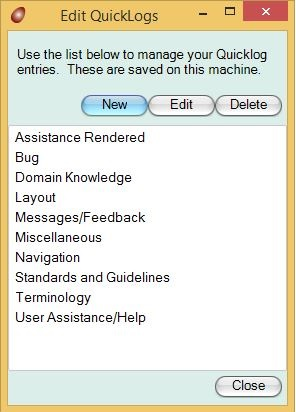
\includegraphics{figures/ovosolo_edit.jpg}
\caption{Ovo Solo note submission window}
\label{fig:ovosolo_edit}
 \end{figure}

This study would have a lot of disadvantages in the scope of our research. The solution doesn't provide means to mark the continuous phases of project development, so it would require an additional work for the researcher to go through the data and either distinguish which highlights represent which engineering process, either group the QuickLog events according to the activities. Lack of configuration abilities of the predefined feedback options would leave the researcher with either small amount of information or a lot of plain text which needs to be processed. The solution doesn't include any means to process the observations and extract information out of the data.\\

As the solution doesn't provide surveys, and there will be some other means to gather the survey data, the data will be separated and it will require more time and effort to combine the results from different sources. Also if the experiment is designed to conduct all the surveys at the end of the experiment, the results will be worse as people tend to forget and it's better to gather feedback right after the end of the activity. If the experiment is designed for the participants to fill the surveys during the experiment according to the development phase or activity, it will require more effort from the researcher or the participants to navigate from one software to another at the proper moments. Giving the participants the freedom to turn off and on the recording might on one hand bring more comfort to the users, on the other hand some of the important data can be lost. As the solution is Windows specific, it's not possible to conduct the experiment on neither Mac nor Linux based OS.\\

This approach wouldn't allow the smooth flow of the experiment as either the researcher or the participants will have to navigate between different programs. Moreover there will be a huge problem with the synchronization of data collected by different sources, let alone synchronization of the recordings of different session within one experiment. \\ 

\section{Distinction with our solution }\label{section:distinction}

The solution presented in the thesis is smoothly integrated into the workbench not as an external tool, but as inner module, works with its code, uses the classes and inner system of logging and event handling. It makes the solution sensitive to the inner processes and events of the workbench. It's possible to configure the solution to react to certain situations and study usage patterns, collect situation-specific feedback, etc.\\

The integrated solution simplifies the organization and the flow of the experiment. Neither the researcher nor the participants would need to install, configure or navigate to any other software except of the workbench. The configuration of the experiment includes configuration of the bookmarks, questionnaires and custom event triggers. It has everything needed for the evaluation of MaCon approach, is designed for the manufacturing engineering project development and doesn't contain redundant complex functionality or require any additional software installation and configuration except the configuration of the surveys, bookmarks and triggers.\\ 

There are different types of bookmarks and opportunity to fold them that fits the possibility of covering complicated non-consequential engineering processes. The software has no problems responding to the need of repeatable activities, what happens during the iterative engineering process. Additional advantage of the solution are the automatic triggers of events that submit certain bookmarks and can call certain questionnaires. The configuration of those is flexible and integrates with the inner logic of the workbench software. \\

The experiment results are synchronized, processed and displayed by the Analysis Tool in the way needed for engineering tool and approach evaluation. It has players and timelines to run the recordings for the retrospective analysis and bookmarks to show the events and activities. The tool is adjusted for handling multiple sessions of participants who are collaboratively working in the software on the project during concurrent engineering. The Analysis Tool displays the data from the surveys and provides the functionality to clusterize and therefore process feedback in the form of plain text into charts, which makes it easier to extract knowledge out of plain text feedback and capture the result.